\documentclass[11pt]{article}
\input{../calcnotes.sty}
\fancyhead[C]{2.1 Rates of Change and Limits}

\begin{document}

\noindent Today, we start working on Calculus-like things. The first of which is a limit. Limits will come up repeatedly all year! They are difficult to understand (sometimes), but not difficult to work with.\\[2ex]

\noindent To illustrate, how do we calculate average velocity? Start by saying $\displaystyle y = f(t)$ and $\displaystyle y$ is a position or distance function. Average velocity is\dots\\[2ex]

\noindent If the displacement function of a falling object is $\displaystyle y=16t^2$, find the average speed over the first $\displaystyle 2$ seconds.\\[2ex]

\noindent Now for the Calculus part, how do we find the \emph{instantaneous speed}---that is, the speed at any \emph{instant}? Look at the average speed formula:\\[2ex]

\noindent We want to calculate this as $\displaystyle h$ gets closer and closer to zero (we can't divide by zero, can we?).\\[2ex]

\noindent Use the example above to find the instantaneous velocity at $\displaystyle t = 2$ seconds.\\[2ex]

\noindent Ok, that works well in this case. Let's write and solve a more difficult one\dots

\[\lim_{x\to0} \frac{\sin x}{x} =\]\\[2ex]

\noindent We need a definition (Calculus likes these; it is very theory-based).\\
Assume $\displaystyle f$ is defined in a neighborhood of $\displaystyle c$ and let $\displaystyle c$ and $\displaystyle L$ be real numbers. The function $\displaystyle f$ has the limit $\displaystyle L$ as $\displaystyle x$ approaches $\displaystyle c$ if, given any positive number $\displaystyle \varepsilon$, there is a positive number $\displaystyle \delta$ such that for all $\displaystyle x$:\\[1ex]

\noindent $\displaystyle 0 < |x - c| < \delta \Rightarrow |f(x) - L| < \varepsilon$, we write $\displaystyle \lim_{x\to c} f(x) = L$\\[2ex]

\noindent Examples help here\dots\\
Graph $\displaystyle f(x) = \frac{x^2 - 1}{x - 1}$,
$g(x) = \begin{cases}
        \frac{x^2 - 1}{x - 1}, & x \neq 1 \\[1ex]
        1,                     & x = 1
    \end{cases}$, $\displaystyle h(x) = x + 1$

\vspace{1ex}

\begin{center}
    \begin{minipage}{0.32\textwidth}
        \centering $\displaystyle f(x)$\\[3pt]
        \smallgraph
    \end{minipage}
    \begin{minipage}{0.32\textwidth}
        \centering $\displaystyle g(x)$\\[3pt]
        \smallgraph
    \end{minipage}
    \begin{minipage}{0.32\textwidth}
        \centering $\displaystyle f(x)$\\[3pt]
        \smallgraph
    \end{minipage}
\end{center}

\noindent Find the limit for each function as $\displaystyle x$ approaches 1.\\[2ex]

\noindent We define some properties of limits with $\displaystyle L$, $\displaystyle M$, $\displaystyle c$, and $\displaystyle k$ as real numbers and $\displaystyle \lim_{x\to c} f(x) = L$ and $\displaystyle \lim_{x\to c} g(x) = M$:
\begin{itemize}
    \item Sum Rule: $\displaystyle \lim_{x\to c}(f(x) + g(x)) = L + M$
    \item Difference Rule: $\displaystyle \lim_{x\to c}(f(x) - g(x)) = L - M$
    \item Product Rule: $\displaystyle \lim_{x\to c}(f(x) \cdot g(x)) = L \cdot M$
    \item Constant Multiple Rule: $\displaystyle \lim_{x\to c}(k \cdot f(x)) = k \cdot L$
    \item Quotient Rule: $\displaystyle \lim_{x\to c}\frac{f(x)}{g(x)} = \frac{L}{M},\ M \neq 0$
\end{itemize}

\vspace{2ex}

\noindent Most of these are common sense, but they pop up often. Find the limits:

\begin{align*}
    \lim_{x\to3}[x^2(2-x)] &  & \lim_{x\to0}\frac{\tan x}{x} &  & \lim_{x\to1}\frac{x^2 - 3x + 2}{x^2 - 1}
\end{align*}\\[2ex]

\noindent It is important to remember that you can only find a limit if it approaches the same thing from \emph{both} sides. See if you can find: $\displaystyle \lim_{x\to2}\frac{x^3 - 1}{x - 2}$\\[2ex]

\noindent This bugs some people, so we say, ``Fine, we can also find it from just one side:''

\begin{align*}
    \lim_{x\to 0^-} = &  & \lim_{x\to 0^+} = \\
    \lim_{x\to 0} =
\end{align*}

\noindent To illustrate, look at this diagram:

\noindent
\begin{minipage}{0.45\textwidth}
    \begin{align*}
        \lim_{x\to 1^-} f(x) & = \underline{\hspace{1cm}} & \lim_{x\to 1^+} f(x) & = \underline{\hspace{1cm}} \\[1ex]
        \lim_{x\to 2^-} f(x) & = \underline{\hspace{1cm}} & \lim_{x\to 2^+} f(x) & = \underline{\hspace{1cm}}
    \end{align*}
\end{minipage}
\hfill
\begin{minipage}{0.5\textwidth}
    \centering
    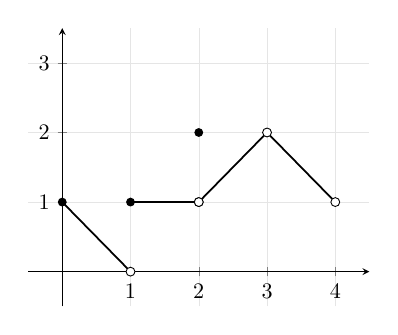
\begin{tikzpicture}[scale=0.8]
        \begin{axis}[
                axis lines = center,
                xmin=-0.5, xmax=4.5,
                ymin=-0.5, ymax=3.5,
                xtick={1,2,3,4},
                ytick={1,2,3},
                grid = both,
                grid style={line width=.1pt, draw=gray!20},
                width=7cm, height=6cm,
                clip=false
            ]
            \addplot[domain=0:1, samples=2, thick, black] {-x + 1};
            \fill[black] (axis cs:0,1) circle (2pt);
            \draw[black, fill=white] (axis cs:1,0) circle (2pt);

            \addplot[domain=1:2, samples=2, thick, black] {1};
            \fill[black] (axis cs:1,1) circle (2pt);
            \draw[black, fill=white] (axis cs:2,1) circle (2pt);

            \fill[black] (axis cs:2,2) circle (2pt);

            \addplot[domain=2:3, samples=2, thick, black] {x - 1};
            \draw[black, fill=white] (axis cs:2,1) circle (2pt);
            \fill[black] (axis cs:3,2) circle (2pt);

            \addplot[domain=3:4, samples=2, thick, black] {-x + 5};
            \draw[black, fill=white] (axis cs:3,2) circle (2pt);
            \draw[black, fill=white] (axis cs:4,1) circle (2pt);
        \end{axis}
    \end{tikzpicture}
\end{minipage}

\vspace{1ex}

\noindent Finally, something called the (seriously) Sandwich Theorem. Don't worry too much about this one (there will be more later).\\[0.5cm]
Show that $\displaystyle \lim_{x\to0}\left[x^2\sin\!\left(\frac{1}{x}\right)\right]=0$.

\end{document}
